
The goal of the advanced IMP utilization for OZG is to improve upon the solution presented in chapter 4 while allowing it to be modify and replace large portions of the existing system architecture. 

\section{IMP Solution Integration}

\subfile{13-imp_solution_integration}

\section{Technological Integration}

\subfile{14-technological_integration}

\subsection{Solution Evaluation}

\begin{itemize}

    \item The IMP solution present in this chapter reduces the amount of systems processing personal information to the absolute minimum: only the responsible institution and the user.
    
    \item The integration architecture described in section 4.2 was able to integrate into two different system architectures. This demonstrates, that the presented integration architecture is applicable to a variety of system architectures.
    
    \item The integration architecture described in section 4.2 was able to integrate a user oriented (persistent) relationship scenario as well as a process oriented (temporary) relationship scenario. This demonstrates, that the presented integration architecture can be used for integrating a variety of IMP solutions.
    
    \item The modular message based approach made it possible to use the integration architecture in a different scenario, by enabling easy configuration of modules for new requirements.
    
    \item IMP utilization of chapter 5 can be used simultaneously to IMP utilization of chapter 4 or as an incremental step.
    
    \item Eventually, profile based operation of OZG can be replaced by process based IMP solution.
    
\end{itemize}

\begin{center}
    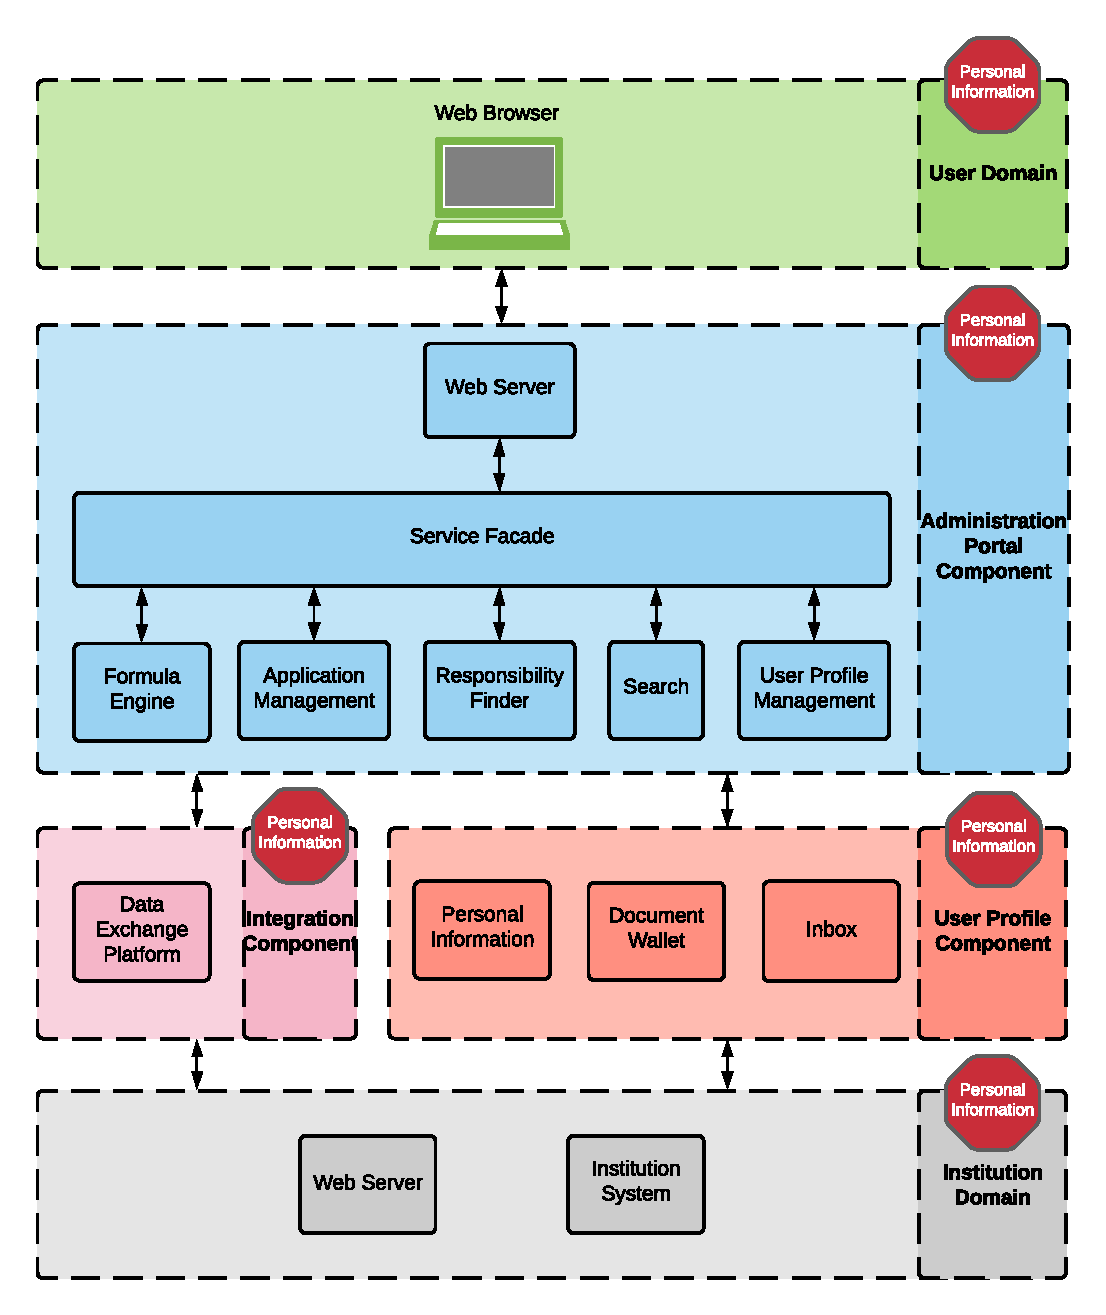
\includegraphics[scale=0.6]{Diagrams/Integration Architecture 2/OZG Personal Information.pdf}
\end{center}

\begin{center}
    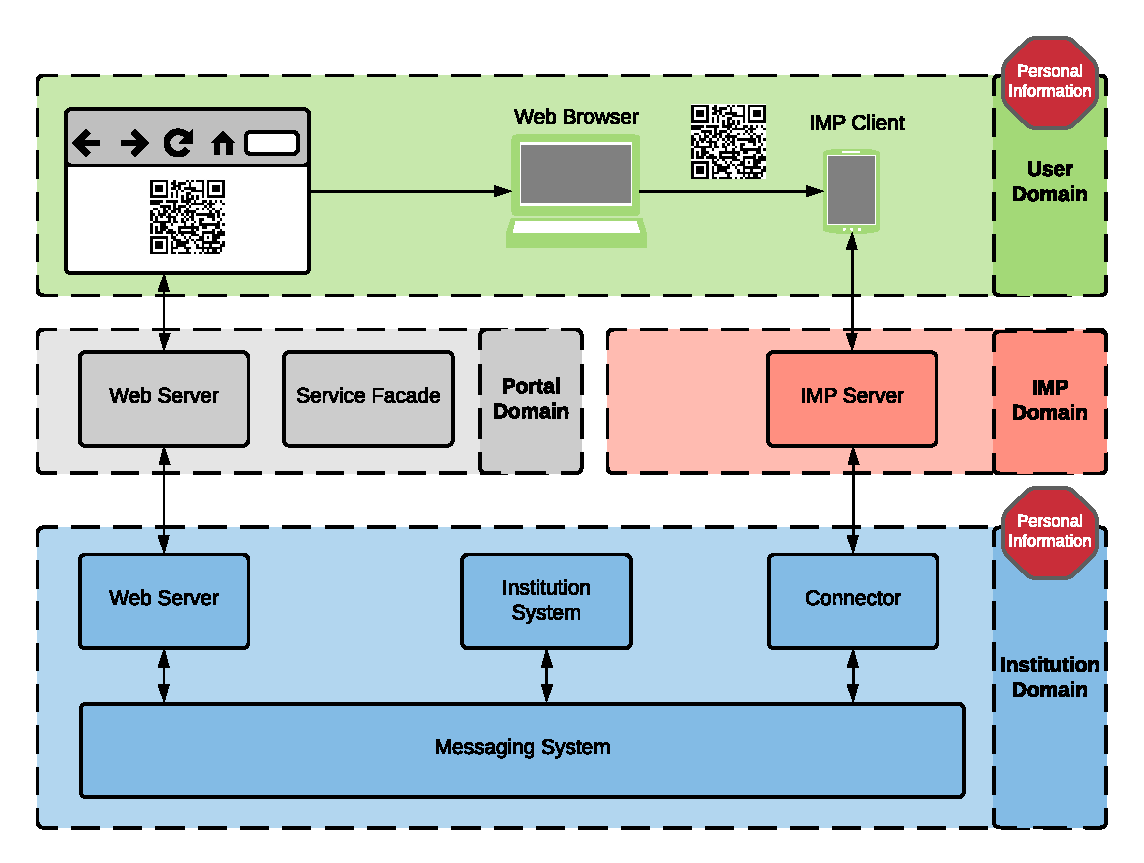
\includegraphics[scale=0.6]{Diagrams/Integration Architecture 2/IMP Personal Information.pdf}
\end{center}